\documentclass[a4paper]{article}

\usepackage[a4paper, top=8mm, bottom=8mm, left=8mm, right=8mm]{geometry}

\usepackage{polyglossia}
\setdefaultlanguage[babelshorthands=true]{russian}
\setotherlanguage{english}

\usepackage{fontspec}
\setmainfont{FreeSerif}
\newfontfamily{\russianfonttt}[Scale=0.7]{DejaVuSansMono}

\usepackage[tiny, compact]{titlesec}

\usepackage{titling}
\setlength{\droptitle}{-1cm}
\pretitle{\begin{center}\begin{bfseries}\Large}
\posttitle{\par\end{bfseries}\end{center}}
\preauthor{\begin{center}\normalsize}
\postauthor{\par\end{center}\vspace{-1.8cm}}

\usepackage{hyperref}
\usepackage{bookmark}
\usepackage{csquotes}
\usepackage{graphicx}


\title{Экспериментальное исследование методов оптимизации умножения плотных матриц на графических процессорах с использованием OpenCL}

\author{Грезин Данил Максимович}

\date{}

\begin{document}
\maketitle
\begin{flushright}
\begin{tabular}{r}
    Группа: \emph{\enquote{25.Б41-мм}} \\
    Кафедра: \emph{системного программирования} \\
    Научный руководитель: \emph{Григорьев Семен Вячеславович} \\
    Номер семестра практики: \emph{2} \\
\end{tabular}
\end{flushright}

\section{Постановка задачи}

Умножение плотных матриц с элементами одинарной точности (стандартный 32-битный формат представления чисел с плавающей точкой) является одной из наиболее важных вычислительных операций в высокопроизводительных вычислениях, поэтому производительность многих приложений напрямую зависит от производительности реализации данной операции на графических процессорах.

Работа выполнялась в рамках учебного исследования методов оптимизации вычислений на графическом процессоре NVIDIA GeForce RTX 4060 с использованием OpenCL (Open Computing Language)\footnote{The Khronos Group. Обзор OpenCL. URL: \url{https://www.khronos.org/opencl/} (дата обращения: 08.03.2026).}~--- стандарта разработки программ для выполнения параллельных вычислений. Исследование проводилось на основе существующего набора реализаций умножения матриц. Реализации отличаются применяемыми методами повышения производительности, направленными на сокращение числа обращений к памяти, повышение эффективности использования локальной памяти и регистров, а также изменение распределения вычислений между потоками.

\textbf{Целью работы является} экспериментальное исследование влияния различных методов оптимизации умножения плотных матриц на производительность вычислений при их выполнении на графическом процессоре.

Результаты работы позволяют оценить влияние отдельных оптимизаций на производительность вычислений. Полученные данные могут использоваться для выбора параметров реализации умножения матриц, оптимальных по критерию максимального среднего значения производительности на конкретном графическом процессоре.

Для достижения поставленной цели были решены следующие задачи:
\begin{itemize}
\item провести экспериментальное исследование производительности различных реализаций умножения матриц, представленных в проекте myGEMM\footnote{Cedric Nugteren. Репозиторий проекта myGEMM. URL: \url{https://github.com/CNugteren/myGEMM} (дата обращения: 10.03.2026).};
\item проанализировать влияние отдельных методов оптимизации, используемых в реализациях умножения матриц, на производительность выполнения вычислений на графическом процессоре;
\item автоматизировать подбор параметров оптимизации;
\item определить значения параметров, обеспечивающие максимальное среднее значение производительности для используемого графического процессора и сравнить их со значениями, предлагаемыми в проекте myGEMM по умолчанию.
\end{itemize}

\section{Описание предлагаемого решения}

В качестве основы для выполнения работы был использован проект myGEMM, реализующий набор методов оптимизации умножения матриц с использованием OpenCL.

В проекте myGEMM представлено 11 вариантов вычислительных ядер, каждое из которых реализует новый метод оптимизации умножения матриц. Наличие нескольких реализаций позволяет проследить влияние методов оптимизации на производительность вычислений на графическом процессоре и делает проект myGEMM удобной платформой для их экспериментального исследования.

Для отдельных реализаций предусмотрены настраиваемые параметры, влияющие на организацию вычислений. При умножении матриц вычисляемая область результирующей матрицы разбивается на вычислительные блоки, каждый из которых обрабатывается группой потоков. Размер такого блока задается параметром TS (Tile Size). Параметр WPT (Work Per Thread) определяет, сколько элементов результирующей матрицы вычисляет один поток, позволяя изменять соотношение между количеством потоков и объемом работы каждого из них. Параметр WIDTH определяет количество элементов, обрабатываемых одной векторной операцией. Для более детальной настройки отдельных реализаций используются параметры TSM, TSN и TSK, задающие размеры обрабатываемых блоков по измерениям M, N и K соответственно, где M и N соответствуют размерам строк и столбцов результирующей матрицы, а K~--- размеру внутреннего измерения, по которому выполняется суммирование при умножении матриц. Параметры WPTM и WPTN определяют количество элементов результирующей матрицы, вычисляемых одним потоком, по измерениям M и N соответственно. Изменение данных параметров может существенно влиять на достигаемую производительность.

В рамках работы были разработаны программы на языке Python, обеспечивающие автоматический запуск вычислительных ядер, сбор результатов измерений, их статистическую обработку и подбор параметров, обеспечивающих максимальное среднее значение производительности.

Работа программ организована следующим образом. На этапе настройки формируется набор параметров для запуска вычислительных ядер. При автоматическом подборе производится перебор допустимых комбинаций параметров с проверкой ограничений, связанных с особенностями графического процессора и конкретной реализацией ядра. Для каждой конфигурации выполняется сборка проекта с выбранными параметрами, после чего производится серия запусков программы и извлечение полученных значений производительности из ее вывода. Полученные результаты сохраняются и используются для последующей статистической обработки. На основе результатов измерений вычисляются статистические характеристики и выбирается конфигурация, обеспечивающая максимальное среднее значение производительности. Все программы расположены в корневом каталоге проекта, разработанного в рамках данной работы:

\begin{itemize}
\item \texttt{run\_experiments\_default.py}~--- запуск измерений с параметрами по умолчанию для каждого ядра;
\item \texttt{run\_experiments\_tuned.py}~--- перебор всех допустимых комбинаций параметров для каждого ядра с проверкой ограничений (объем памяти, делимость значений);
\item \texttt{calculate\_results\_default.py}~--- статистическая обработка результатов по умолчанию: расчет среднего, стандартного отклонения, 95\%-го доверительного интервала, проверка нормальности распределения;
\item \texttt{calculate\_results\_tuned.py}~--- статистическая обработка результатов с перебором параметров и выбор лучшей конфигурации по наибольшему среднему значению производительности.
\end{itemize}

Для проверки корректности разработанных программ были написаны модульные тесты с использованием \texttt{pytest}\footnote{pytest development team. Документация pytest. URL: \url{https://docs.pytest.org/en/stable/} (дата обращения: 20.04.2026).}, размещенные в директории \texttt{tests/unit/}. Тесты охватывают корректность функций проверки подбираемых параметров, статистической обработки результатов и обработки выбросов.

\section{Экспериментальное исследование производительности}

С использованием разработанных программ были проведены измерения производительности всех ядер проекта myGEMM. Для каждого ядра выполнялось измерение стандартной конфигурации, использующей параметры, заданные в исходном проекте myGEMM. Для ядер, поддерживающих настройку параметров, дополнительно проводилось сравнение с оптимизированной конфигурацией, полученной в результате автоматического подбора параметров по критерию максимального среднего значения производительности. Для ядер, не имеющих настраиваемых параметров, исследование ограничивалось измерением стандартной конфигурации.

Целью экспериментального исследования является оценка влияния методов оптимизации и автоматического подбора параметров вычислительных ядер на производительность умножения плотных матриц при выполнении вычислений на графическом процессоре.

Эксперименты проводились на следующей конфигурации вычислительной системы:
\begin{itemize}
\item процессор AMD Ryzen 7 7435HS (8 ядер, 16 потоков);
\item оперативная память 16 ГБ;
\item графический процессор NVIDIA GeForce RTX 4060 Laptop GPU (8 ГБ);
\item операционная система Manjaro Linux;
\item драйвер NVIDIA 590.48.01;
\item CUDA Toolkit 13.1;
\item NVCC 13.1.115;
\item OpenCL 3.0;
\item компилятор GCC 15.2.1;
\item флаги компиляции \texttt{-O3 -arch=sm\_89 -Xcompiler -Wall}.
\end{itemize}

Для каждой конфигурации выполнялось 40 измерений производительности после серии предварительных запусков. Между компиляциями и сменами размеров матриц делалась пауза для стабилизации температурного режима графического процессора. В качестве исследуемой задачи использовалось умножение квадратных матриц размеров \(8192 \times 8192\) и \(8320 \times 8320\). Размер 8192 выбран как достаточно большое значение, являющееся степенью двойки и позволяющее исследовать производительность вычислительных ядер при больших объемах вычислений. Размер 8320 выбран как близкое по величине значение, не являющееся степенью двойки, для проверки ядер, поддерживающих обработку матриц произвольного размера. По результатам измерений вычислялись среднее значение производительности, стандартное отклонение и 95\%-й доверительный интервал, а также выполнялась проверка нормальности распределения результатов с использованием тестов Д'Агостино и Шапиро-Уилка.

Время выполнения каждого измерения определялось с использованием функции \texttt{gettimeofday}, обеспечивающей получение времени в секундах. Каждый элемент результирующей матрицы при умножении плотных квадратных матриц размера \(N \times N\) вычисляется как скалярное произведение строки и столбца длины \(N\), что требует выполнения \(N\) операций умножения и \(N\) операций сложения. Таким образом, для вычисления одного элемента выполняется \(2N\) арифметических операций, а для всей результирующей матрицы, содержащей \(N^2\) элементов,~--- \(2N^3\) операций. Производительность измеряется в GFLOPS (Giga Floating-point Operations Per Second) как число арифметических операций с числами с плавающей точкой в секунду, где 1 GFLOPS соответствует $10^9$ операциям в секунду. Итоговая производительность вычислялась по формуле:
\[
GFLOPS = \frac{2N^3}{t \cdot 10^9},
\]
где \(t\)~--- время выполнения одного измерения в секундах.

Результаты измерений для стандартной конфигурации, а также после автоматического подбора параметров, обеспечивающих максимальное среднее значение производительности, представлены на странице репозитория в файле \texttt{README.md}.

Сравнение производительности ядер до и после подбора параметров для исследуемых размеров матриц приведено на рисунке~\ref{fig:kernel-comparison}. На горизонтальной оси графика представлено среднее значение производительности в GFLOPS, вычисленное по результатам серии измерений, а на вертикальной оси~--- названия вычислительных ядер проекта myGEMM с указанием размера матриц и используемой конфигурации параметров. Вариант <<default>> соответствует параметрам, заданным в исходном проекте myGEMM. Вариант <<tuned>> соответствует конфигурации, полученной в результате автоматического подбора допустимых комбинаций параметров ядра и обеспечивающей максимальное среднее значение производительности среди рассмотренных вариантов. Для некоторых ядер на графике представлен только вариант <<default>>. Это связано либо с отсутствием настраиваемых параметров, допускающих автоматический подбор конфигурации, либо с тем, что подбор параметров не привел к увеличению среднего значения производительности. Бордовым цветом показаны результаты выполнения с использованием CUDA (Compute Unified Device Architecture)\footnote{NVIDIA. CUDA Toolkit Documentation. URL: \url{https://docs.nvidia.com/cuda/} (дата обращения: 10.03.2026).}~--- платформы для разработки программ, выполняющих параллельные вычисления на графических процессорах. Малиновым цветом показаны результаты выполнения с использованием OpenCL. Белыми отрезками обозначено стандартное отклонение результатов измерений.

\begin{figure}[htbp]
    \centering
    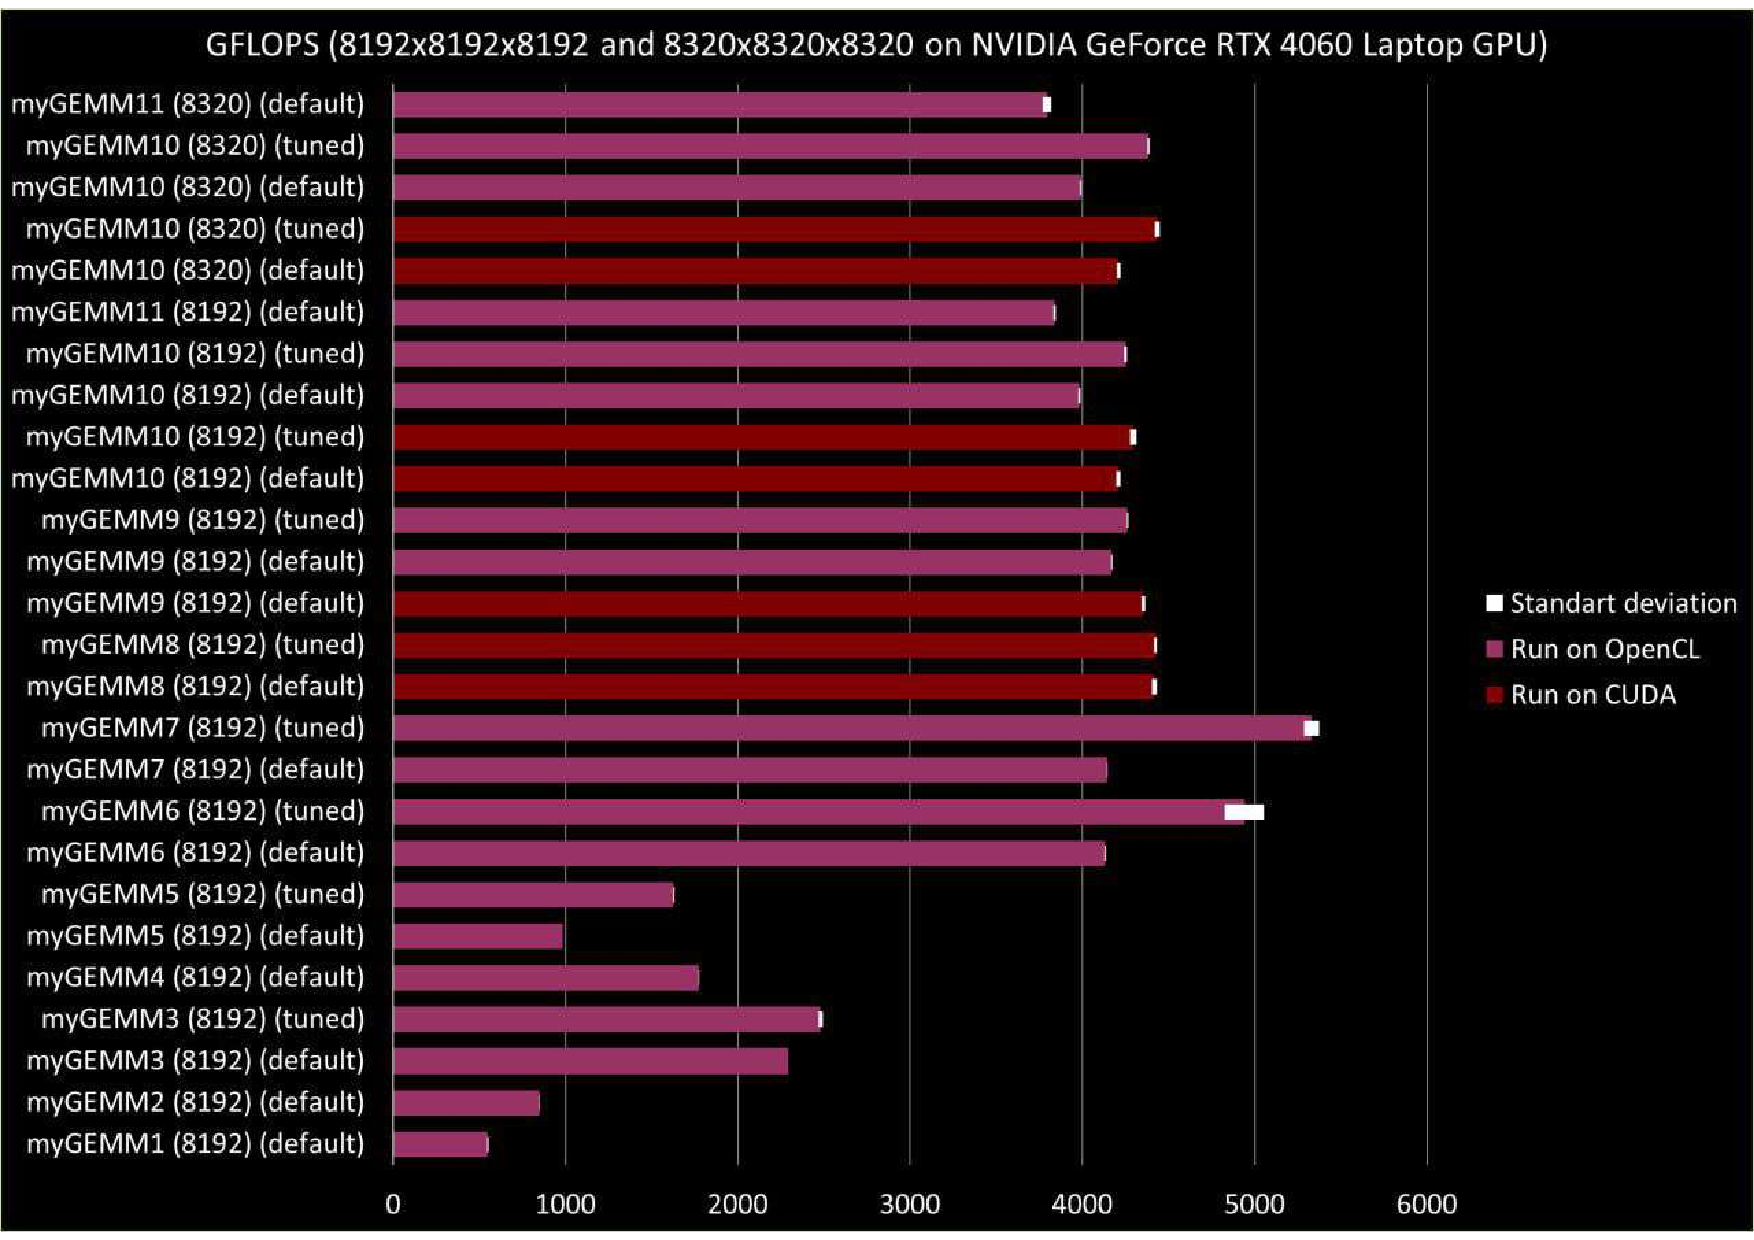
\includegraphics[width=0.7\textwidth]{kernel_comparison.pdf}
    \caption{Производительность вычислительных ядер до и после подбора параметров}
    \label{fig:kernel-comparison}
\end{figure}

В ходе эксперимента были выявлены следующие ядра, показавшие наибольший прирост производительности после оптимизации параметров:

\begin{itemize}
\item ядро 5~--- прирост производительности около 65\% за счет увеличения размера вычислительного блока (TS с 32 до 64) и объема работы на поток (WPT с 8 до 16);
\item ядро 6~--- прирост производительности около 20\% за счет увеличения размера вычислительного блока по измерению K (TSK с 16 до 32);
\item ядро 7~--- прирост производительности около 29\% за счет уменьшения ширины вектора (WIDTH с 4 до 2).
\end{itemize}

Остальные ядра (1, 2, 3, 4, 8, 9, 10, 11) не показали заметного изменения производительности. Их параметры, заданные в исходном проекте myGEMM, уже обеспечивали максимальное или близкое к максимальному среднее значение производительности для используемой видеокарты среди рассмотренных конфигураций.

Полученные результаты подтверждают, что учет особенностей конкретного графического процессора при подборе параметров вычислительных ядер позволяет в ряде случаев существенно повысить производительность без изменения алгоритма вычислений.

\section{Заключение}

В ходе выполнения работы получены следующие результаты:

\begin{itemize}
    \item разработаны программы для автоматизированного запуска измерений (\texttt{run\_experiments\_default.py}, \texttt{run\_experiments\_tuned.py}) и статистической обработки результатов (\texttt{calculate\_results\_default.py}, \texttt{calculate\_results\_tuned.py});
    \item написаны модульные тесты для проверки корректности скриптов (\texttt{tests/unit/});
    \item проведены измерения производительности 11 вычислительных ядер в стандартной и оптимизированной (для ядер, поддерживающих настройку параметров) конфигурациях на матрицах размером \(8192 \times 8192\) и \(8320 \times 8320\);
    \item выполнен автоматический перебор параметров и определены конфигурации, обеспечивающие максимальное среднее значение производительности для NVIDIA GeForce RTX 4060.
\end{itemize}

Репозиторий: \url{https://github.com/Snaffys/myGEMM}.

Техническая документация, описание методики проведения экспериментов, а также результаты измерений и графики производительности представлены в файле \texttt{README.md} репозитория.

Полученные результаты демонстрируют практическую значимость автоматического подбора параметров вычислительных ядер, позволяющего повысить производительность вычислений на графическом процессоре без изменения алгоритма умножения матриц.
\end{document}
